\documentclass[a4paper,12pt]{article}
 
%% Начало шапки
 
%% Настройка поддержки русского языка
\usepackage{cmap}                   % Поиск по кириллице
\usepackage{mathtext}               % Кириллица в формулах
\usepackage[T1,T2A]{fontenc}        % Кодировки шрифтов
\usepackage[utf8]{inputenc}         % Кодировка текста
\usepackage[english,russian]{babel} % Подключение поддержки языков
 
%% Настройка размеров полей
\usepackage[top=0.7in, bottom=0.75in, left=0.625in, right=0.625in]{geometry}
 
%% Математические пакеты
\usepackage{mathtools}              % Тот же amsmath, только с некоторыми поправками
\usepackage{amssymb}                % Математические символы
\usepackage{amsthm}                 % Оформление теорем
\usepackage{amstext}                % Текстовые вставки в формулы
\usepackage{amsfonts}               % Математические шрифты
\usepackage{icomma}                 % "Умная" запятая: $0,2$ --- число, $0, 2$ --- перечисление
\usepackage{enumitem}               % Для выравнивания itemize (\begin{itemize}[align=left])
\usepackage{array}                  % Таблицы и матрицы
\usepackage{multirow}
 
%% Алгоритмические пакеты и их настройки
\usepackage{algorithm}              % Шапка алгоритма
\usepackage{algorithmicx}           % Написание алгоритмов
\usepackage[noend]{algpseudocode}   % Написание псевдокода; убраны end
\usepackage{listings}               % Для кода на каком-либо языке программиования
\renewcommand{\algorithmicrequire}{\textbf{Ввод:}}              % Ввод
\renewcommand{\algorithmicensure}{\textbf{Вывод:}}              % Вывод
\floatname{algorithm}{Алгоритм}                                 % Название алгоритма
\renewcommand{\algorithmiccomment}[1]{\hspace*{\fill}\{// #1\}} % Комментарии
\newcommand{\algname}[1]{\textsc{#1}}                           % Вызов функции в алгоритме
\usepackage{physics}
 
%% Шрифты
\usepackage{euscript}               % Шрифт Евклид
\usepackage{mathrsfs}               % \mathscr{}
 
%% Графика
\usepackage[pdftex]{graphicx}       % Вставка картинок
\graphicspath{{images/}}            % Стандартный путь к картинкам
\usepackage{tikz}  
\usetikzlibrary{patterns}                 % Рисование всего
\usepackage{pgfplots}               % Графики
 
%% Прочие пакеты
\usepackage{indentfirst}                    % Красная строка в начале текста
\usepackage{epigraph}                       % Эпиграфы
\usepackage{fancybox,fancyhdr}              % Колонтитулы
\usepackage[colorlinks=true, urlcolor=blue]{hyperref}   % Ссылки
\usepackage{titlesec}                       % Изменение формата заголовков
\usepackage[normalem]{ulem}                 % Для зачёркиваний
\usepackage[makeroom]{cancel}               % И снова зачёркивание (на этот раз косое)

 
%% Прочее
\mathtoolsset{showonlyrefs=true}        % Показывать номера только у тех формул,
                                        % на которые есть \eqref{} в тексте.
\renewcommand{\headrulewidth}{1.8pt}    % Изменяем размер верхнего отступа колонтитула
\renewcommand{\footrulewidth}{0.0pt}    % Изменяем размер нижнего отступа колонтитула

%Прочее
\usepackage{forest} % Деревья

\usetikzlibrary{arrows,calc}
\usetikzlibrary{quotes,angles}

\usetikzlibrary{positioning,intersections}

\usetikzlibrary{through}

\NewDocumentCommand{\bissectrice}{%
	O{}     % drawing options
	mmm     % bissector of mmm
	m       % intersection point between base and bissector
	O{1}O{1}% extended drawing of the bissector
}{%
\path[name path=Bis#2#3#4] let
\p1 = ($(#2) - (#3)$),
\p2 = ($(#4) - (#3)$),
\n1 = {veclen(\x1,\y1)/2} ,
\n2 = {veclen(\x2,\y2)/2} ,
\n3 = {max(\n1,\n2)},
\p1 = ($(#3)!\n3!(#2)$),
\p2 = ($(#3)!\n3!(#4)$),
\p3 = ($(\p1) + (\p2) - (#3)$)
in
(#3) -- (\p3) ;

\path[name path = foo] (#2)--(#4) ;

\path[name intersections={of=foo and Bis#2#3#4, by=#5}] ;

\path[#1] ($(#3)!#6!(#5)$) -- ($(#5)!#7!(#3)$) ;
}


\tikzset{
	right angle quadrant/.code={
		\pgfmathsetmacro\quadranta{{1,1,-1,-1}[#1-1]}     % Arrays for selecting quadrant
		\pgfmathsetmacro\quadrantb{{1,-1,-1,1}[#1-1]}},
	right angle quadrant=1, % Make sure it is set, even if not called explicitly
	right angle length/.code={\def\rightanglelength{#1}},   % Length of symbol
	right angle length=2ex, % Make sure it is set...
	right angle symbol/.style n args={3}{
		insert path={
			let \p0 = ($(#1)!(#3)!(#2)$),     % Intersection
			\p1 = ($(\p0)!\quadranta*\rightanglelength!(#3)$), % Point on base line
			\p2 = ($(\p0)!\quadrantb*\rightanglelength!(#2)$), % Point on perpendicular line
			\p3 = ($(\p1)+(\p2)-(\p0)$) in  % Corner point of symbol
			(\p1) -- (\p3) -- (\p2)
		}
	}
}

%% Определения
\newtheorem{definition}{Определение}

\newtheorem*{task}{Задача}
\newtheorem*{task1}{Задача №1}
\newtheorem*{task2}{Задача №2}
\newtheorem*{task3}{Задача №3}
\newtheorem*{task4}{Задача №4}
\newtheorem*{task5}{Задача №5}

\newtheorem{fulllemma}{Лемма}
\newtheorem*{sl1}{Следствие 1}
\newtheorem*{sl2}{Следствие 2}
\newtheorem*{scheme}{Утверждение 1}
\newtheorem*{theorem}{Теорема}
\newtheorem*{proposal}{Предложение}
\newtheorem*{notice}{Замечание}
\newtheorem{statement}{Утверждение}
\newtheorem*{consequence}{Следствие}
\newtheorem*{lemma}{Лемма}

\newcommand{\note}{\underline{Замечание:} }
\newcommand{\fact}{\underline{\textbf{Факт}:} }
\newcommand{\example}{\underline{Пример:} }
\newcommand{\sign}{\underline{Обозначения:} }
\newcommand{\statements}{\underline{Утверждения:} }

\renewcommand{\Re}{\mathrm{Re\:}}
\renewcommand{\Im}{\mathrm{Im\:}}
\newcommand{\Arg}{\mathrm{Arg\:}}
\renewcommand{\arg}{\mathrm{arg\:}}
\newcommand{\Mat}{\mathrm{Mat}}
\newcommand{\id}{\mathrm{id}}
\newcommand{\isom}{\xrightarrow{\sim}} 
\newcommand{\leftisom}{\xleftarrow{\sim}}
\newcommand{\Hom}{\mathrm{Hom}}
\newcommand{\Ker}{\mathrm{Ker}\:}
\newcommand{\rk}{\mathrm{rk}\:}
\newcommand{\diag}{\mathrm{diag}}
\newcommand{\ort}{\mathrm{ort}}
\newcommand{\pr}{\mathrm{pr}}
\newcommand{\vol}{\mathrm{vol\:}}

\newcommand{\Z}{\mathbb{Z}}
\newcommand{\N}{\mathbb{N}}
\newcommand{\Q}{\mathbb{Q}}
\newcommand{\R}{\mathbb{R}}
\renewcommand{\C}{\mathbb{C}}
\renewcommand{\L}{\mathscr{L}}
\renewcommand{\P}{\mathcal{P}}
\newcommand{\p}{\mathsf{p}}
\newcommand{\E}{\mathsf{E}}
\newcommand{\D}{\mathsf{D}}
\newcommand{\cov}{\mathsf{cov}}

\renewcommand{\l}{\mathcal{L}}
\renewcommand{\O}{\mathcal{O}}
\newcommand{\F}{\mathsf{F}}
\renewcommand{\S}{\mathsf{S}}
 
%% Информация об авторах
\title{\Huge{Избранные Главы Линейной Алгебры \\ Факультатив}}
\author{Вадим Гринберг \\ Юрий Баранов}
\date{}

\begin{document}
\maketitle
\tableofcontents


\newpage
\section{Псевдообратная матрица}

\subsection{Свойства}

\subsection{Скелетное разложение}

\subsection{Решение по методу наименьших квадратов}

\newpage
\section{Сингулярное разложение}

\subsection{Суть}

\subsection{Алгоритм построения}


\newpage
\section{Приближённые решения}

\subsection{Псевдорешение СЛУ}

\subsection{Интерполяция}

\subsubsection{Определитель Вандермонда}

\subsubsection{Интеполяционный многочлен Лагранжа}

\subsection{Полиномиальная интерполяция с кратными узлами \\ Многочлен Эрмита}


\newpage
\section{Приближение кривых}

\subsection{Сплайны}

\subsection{Кривые Безье}

\newpage
\section{Метрическое пространство}

\subsection{Метрики, Шары, Сферы}

Пусть $M$ -- некое множество.

\begin{defintion}
	\textbf{Метрика} $\rho$ на множестве $M$ --- это такая функция $\rho (x, y) \geqslant 0$, что 
	\begin{enumerate}
		\item $\rho (x, y) = \rho (y, x)$
		\item $\rho (x, y) > 0, x\neq y, \rho (x, x) = 0$ 
		\item $\rho (x, y) + \rho (y, z) \geqslant \rho (x, z)$
	\end{enumerate}
\end{definition}

\textbf{Примеры}:

\begin{enumerate}
	\item Метрика евклидова пространства $M = \R^n$:
	\[\rho(x,\ y) = \sqrt{\displaystyle\sum\limits_{i = 1}^n(x_i - y_i)^2}\]
	\item Расстояние Хэмминга:
	$M = |\Z_2^n| = \{\vec{x} \mid x_i \in \{0,\ 1\}\}$
	\[\rho(x,\ y) = | i\mid x_i \neq y_i| = \text{кол-во единиц в числе } y - x\]
	\item V
\end{enumerate}



Дана карта с расстояниями между городами.\\
$M$ = \{ города \}\begin{center}
	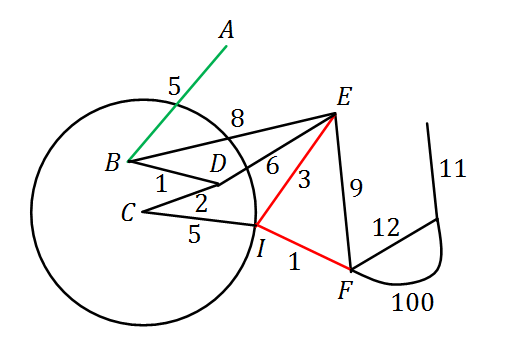
\includegraphics[scale=0.7]{l4_1.png}\end{center}
$\rho (A, B) = 5$\\
$\rho (E, F) = 4$ (минимальное расстояние из возможных)\\
\\
\textbf{Шар в метрическом пространстве.}\begin{center}
	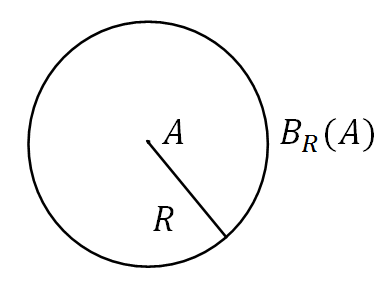
\includegraphics[scale=0.5]{l4_2.png}\end{center}
$B_R(A) = \{x | \rho(A, x) \leqslant R \}$ --- \textbf{шар} радиуса $R$ с центром в точке $A$.\\ 
$S_R(A) = \{x | \rho(A, x) = R \}$ --- \textbf{сфера} радиуса $R$ с центром в точке $A$.\\ 
\\
$B_5(C) = \{ C, B, D, I \}$ --- все точки, которые туда входят. \\
$S_5(C) = \{ I \}$ --- только те точки, которые лежат на окружности. \\
$B_{100}(C) = B_{50} (C) = M $ --- все множество. \\
\\
Метод наименьших квадратов --- приближение функции в смысле следующей метрики \begin{center} $M = \{f: X \rightarrow \mathbb{R} \}, X = \{ x_1, ..., x_n \}$\\ ~\\
	$\rho (f, y) = |\bar y - \bar f| = \sqrt{\sum\limits_{i=1}^n(y(x_i)-f(x_i))^2}$ \\
	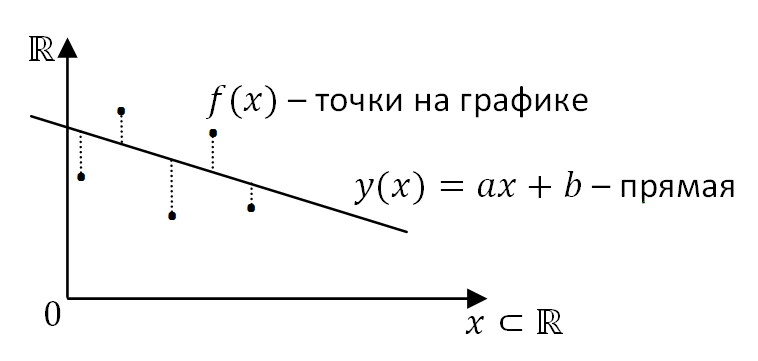
\includegraphics[scale=0.6]{l4_4.png}\end{center}
\noindent \textbf{Пример 1.}\\
Найти такое метрическое пространство $M$, что\\ \\
$  
\left\{  
\begin{array}{lcl}  
B_5(x) \subset B_4(y) \\  
B_5(x) \neq B_4(y)\\
\end{array}   
\right.  
$
, где $x, y$ - две точки. \\ \\То есть доказать, что существует $c\in B_4(y), c\notin B_5(x)$.\begin{center}
	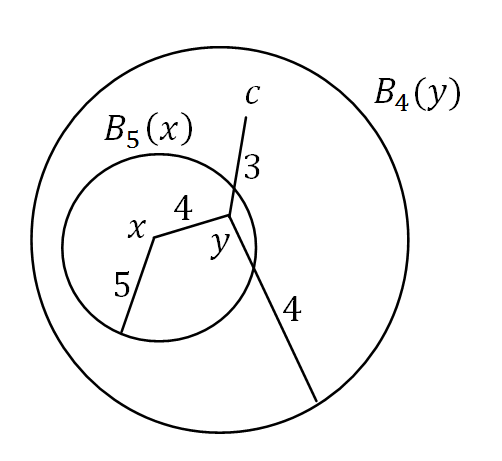
\includegraphics[scale=0.5]{l4_5.png}\\
	$\rho (x, y) = \rho(y, x) = 4$\\
	$\rho (y, c) = \rho(c, y) = 3$\\
	$\rho (x, c) = \rho(c, x) = 7$\\
	~\\
	$B_5(x) = \{ x, y \}$\\
	$B_4(y) = \{x, y, c \} $\end{center}
То есть $B_5(x) \subset B_4(y)$.\\
\\
Вспомним определение линейного пространства.\\
Если на непустом множестве заданы две бинарные операции "+" и "умножение на число", числа из поля $F$, $\forall ~a,~b,~c\in V$ то\begin{enumerate}
	\item $a+(b+c) = (a+b)+c$
	\item $\exists~0: a+0 = 0+a = a$
	\item $\exists~ (-a): a+(-a) = 0$
	\item $a+b = b+a$
	\item $1\cdot x = x$
	\item $ (\mu \lambda)x = \mu(\lambda x)$
	\item $(a+b)\lambda = a\lambda + b\lambda$
	\item $(\mu + \lambda)a = \mu a + \lambda a$
\end{enumerate}
$V$ --- \textbf{линейное пространство} (векторное пространство), если выполнены 8 предыдущих аксиом и \begin{enumerate}
	\item $\forall \bar u, \bar v$: $\bar u + \bar v \in V$
	\item $\forall$ числа $\alpha \in$ $\mathbb{R}$, $\mathbb{C}$ $\alpha \bar u \in V$\\ 
	(или $\alpha \in F$ заданное поле, например, $F_2 = \{ 0, 1 \}$)\end{enumerate}
Линейное пространство $V$ --- \textbf{нормированное}, если на нем задана такая норма \\$\nu : V \to$ $\mathbb{R}$ $\geqslant 0$, что\begin{enumerate}
	\item $\nu(\bar x) > 0$, $\bar x \neq \bar 0$, $\nu(\bar 0) = \bar 0$
	\item $\nu(\alpha \bar x) = |\alpha|\nu(\bar x)$
	\item $\nu(\bar x + \bar y) \leq \nu(\bar x) + \nu(\bar y)$ для $\forall x, y \in V, \forall \alpha$
\end{enumerate}
Из каждой нормы можно сделать метрику $\rho(\bar x, \bar y) = \nu(\bar y - \bar x)$.\\ \\
\textbf{Примеры норм:}\begin{enumerate}
	\item Манхэттенская норма (норма таксиста)\\
	(Можно ехать разными путями, но не по прямой)\begin{center}
		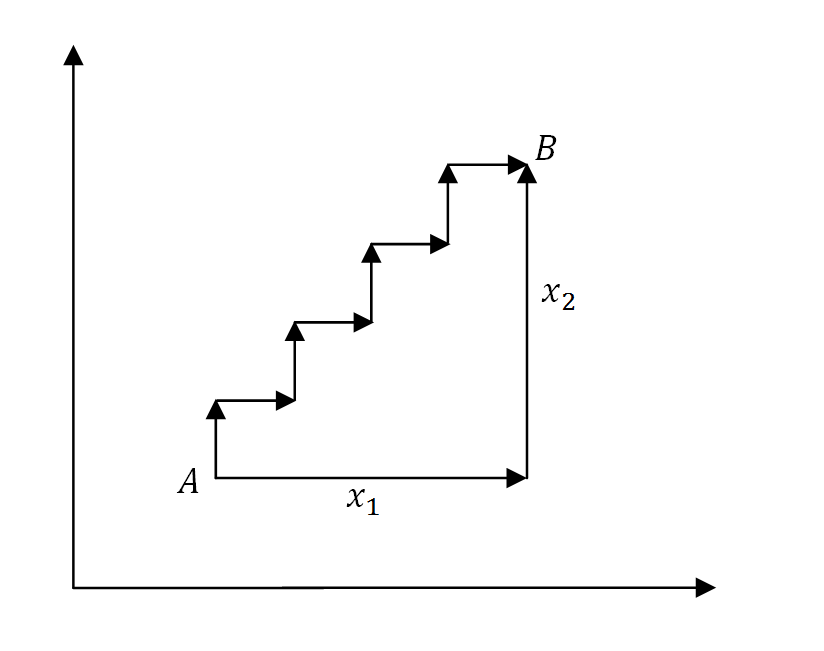
\includegraphics[scale=0.4]{l4_7.png}\end{center}
	\begin{center}$\nu_M(\bar x) = |x_1|+...+|x_n|$ в $\mathbb{R}^n$, где $\bar x = (x_1,..., x_n)$\end{center}
	\item Евклидова норма\\
	(Для приближения)
	\begin{center}
		$\nu_E(\bar x) = \sqrt{|x_1|^2+...+|x_n|^2}$ в $\mathbb{R}^n$\end{center}
	\item Норма максимума\\
	(Уменьшает ошибку по всем координатам)\begin{center}
		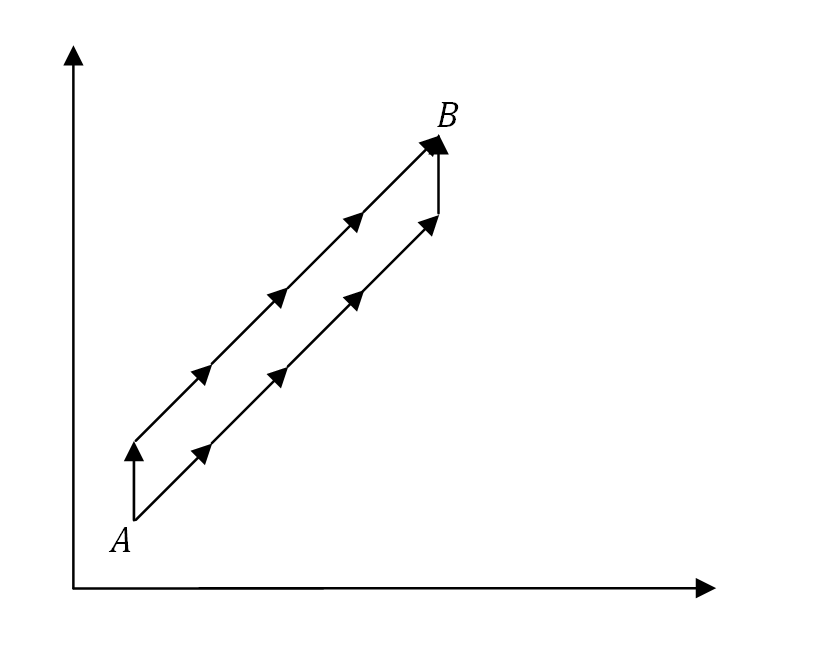
\includegraphics[scale=0.4]{l4_8.png}\end{center}
	\begin{center}
		$\nu_{max}(\bar x) = max\{|x_1|,...,|x_n|\}$ в $\mathbb{R}^n$\\\end{center}
	\item Норма Гёльдера
	\begin{center}$\nu_p(\bar x) = \sqrt[p]{|x_1|^p+...+|x_n|^p}$ в $\mathbb{R}^n$\\
		$\nu_1(\bar x) = |x_1|+...+|x_n| = \nu_M(\bar x)$\\ 
		$\nu_2(\bar x) = \sqrt{|x_1|^2+...+|x_n|^2} = \nu_E(\bar x)$\\
		$\nu_{\infty}(\bar x) = \underset{p \to \infty}{lim}\sqrt[p]{\sum\limits_{i=1}^n |x_i|^p}$\end{center}
	Если $|x_i| = max |x_i|$, то $\sqrt[p]{|x_i|^p} \to |x_i|$, получим:
	\begin{center}$\nu_{\infty}(\bar x) = max \{|x_1|,...,|x_n|\} = \nu_{max}(\bar x)$\end{center}
\end{enumerate}
\textbf{Утверждение.}
В нормированном пространстве $V$ верно:\begin{enumerate}
	\item $\forall \bar x, \bar y ~B_R(\bar x)$ равен $B_R(\bar y)$ (как геометрическая фигура).\\ 
	$\blacktriangleright$ Пусть $\bar v = \bar y - \bar x$, тогда \begin{center} $B_R(\bar y) = \bar v + B_R(\bar x)$\end{center}
	Ко всем точкам из $B_R(\bar x)$ прибавим одинаковый вектор $\bar v$.\begin{center}
		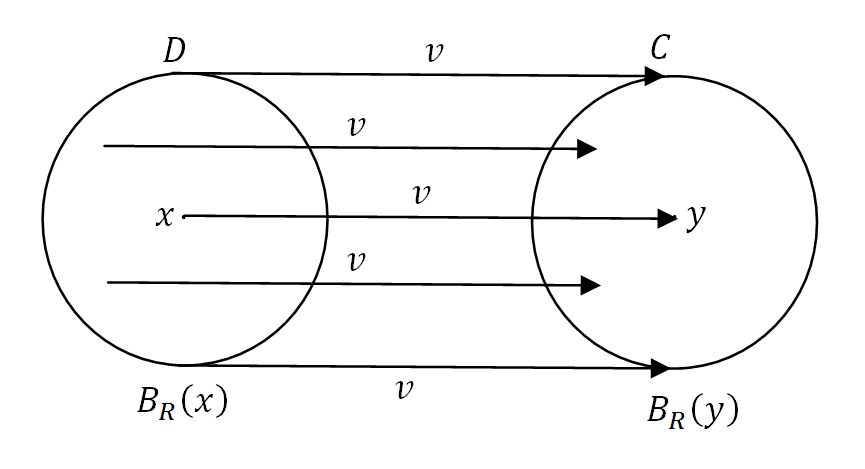
\includegraphics[scale=0.5]{l4_9.png}\\
		$C \in B_R(y) \Leftrightarrow \nu(C-y) \leqslant R$\\
		$\nu((C-(\bar y - \bar x))-\bar x) \leqslant R$\end{center}
	То есть, $D = C-(\bar y-\bar x) \in B_R(\bar x). ~~\blacksquare$
	\item Шары $B_R(\bar x)$ и $ B_{\alpha R}(\bar x)$, $\alpha > 0$ подобны с коэффициентом подобия $\alpha$.\\ 
	$\blacktriangleright$ \begin{center}$\nu(x D) = \cfrac{1}{\alpha}\nu(x C)$\\
		$D = x+xD = x+\cfrac{1}{\alpha}xC$\\
		$\rho(D, x) = \nu(x D) = \cfrac{1}{\alpha}\nu(C-x) = \nu(\cfrac{1}{\alpha}(C-x))$\\
		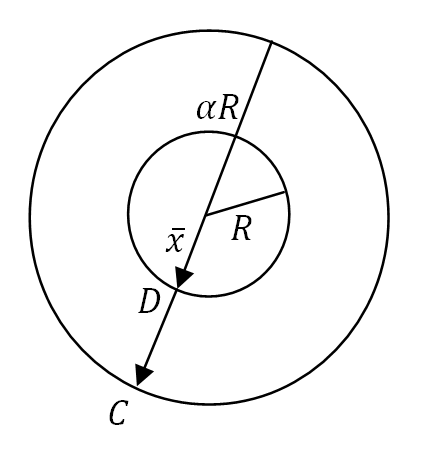
\includegraphics[scale=0.5]{l4_10.png}\\
		$C \in B_{\alpha R}(x) \Leftrightarrow \nu(C-x) \leqslant \alpha R$\\
		$\rho(D, x) = \nu(\cfrac{C-x}{\alpha}) \leqslant R$\end{center} То есть $D \in B_R(\bar x). ~~\blacksquare$
\end{enumerate}
~\\$\nu_p$ --- норма только при $p \geqslant 1$ (для невыпуклых --- неверно, не выполняется неравенство треугольника).\\
$B^p = B_1(\bar 0)$ относительно $\nu_p$.\begin{center}
	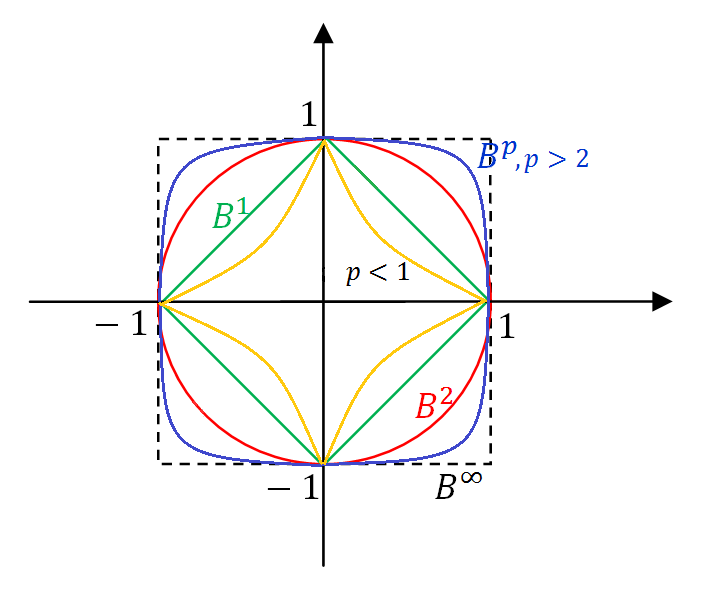
\includegraphics[scale=0.7]{l4_11.png}
	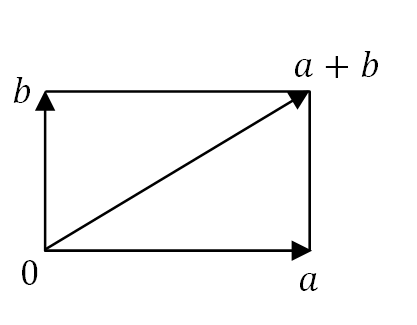
\includegraphics[scale=0.5]{l4_12.png}
\end{center}
\textbf{Пример 2.}\\
Для каких $R_1, R_2$ возможно $B_{R_1}(x) \subsetneq B_{R_2}(y)$?\\
\\
Если $R_2 > R_1$ --- возможно (даже при $x = y$).\\
При $R_1 = 5, R_2 = 4$ --- возможно (из предыдущего примера).\\
Докажем, что при $R_1 > R_2$ это не всегда верно, а именно: при $2R_2 > R_1$ - верно, а при $R_2 \leqslant \cfrac{R_1}{2}$ --- нет.\\
Рассмотрим случай $2R_2 = R_1$. \begin{center}
	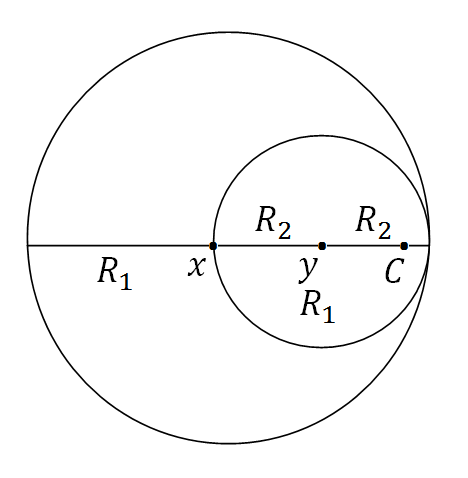
\includegraphics[scale=0.55]{l4_13.png}\end{center}
Тогда $B_{R_1}(x) = \{x, y, C\}$, $B_{R_2}(y) = \{x, y, C\}$, то есть $B_{R_1}(x) = B_{R_2}(y)$ --- множества совпадают, то есть уже не подходит.\\
\\
Рассмотрим случай, когда $R_1$ чуть меньше $2R_2$.\\
Тогда $B_{R_1}(x) = \{x, y\}$, $B_{R_2}(y) = \{x, y, C\}$, то есть $B_{R_1}(x) \subsetneq B_{R_2}(y)$ верно.\\
\\
Рассмотрим случай, когда $R_1$ чуть больше $2R_2$.\\
Тогда $B_{R_1}(x) = \{x, y, C\}$, $B_{R_2}(y) = \{x, y, C\}$, то есть, $B_{R_2}(y) \subseteq B_{R_1}(x)$, значит не подходит.\\
\\
Линейное пространство называется \textbf{евклидовым пространством}, если на нем задано скалярное произведение $g(x, y)$:\begin{enumerate}
	\item $g(x, y) = g(y, x)$
	\item $g(x_1+x_2, y) = g(x_1, y)+g(x_2, y)$
	\item $g(\lambda x, y) = \lambda g(x, y)$
	\item $g(x, x) \geqslant 0, g(x, x) = 0 \Leftrightarrow x = 0$
\end{enumerate}
В евклидовом пространстве есть стандартная норма $\parallel x \parallel = \sqrt{g(x, x)}$.\\
$L_2[0, 1]$ --- множество функций, квадрат которых интегрируем по Риману.\\
$(f, g) = \int\limits_0^1 f(x) \overline{g(x)}\,dx$\\
$\parallel f \parallel_2 = \sqrt{\int\limits_0^1 |f(x)|^2\,dx}$\\
\\
$x_n \to x$ $\textbf{сходится по норме}$ $\nu(x)$, если $\forall \varepsilon > 0 ~ \exists N(\varepsilon)~$, что $\forall n > N(\varepsilon)$ верно $~\nu(x_n - x) < \varepsilon$.\\ \\
\textbf{Пример 3.}\\
Является ли нормой на множестве непрерывно дифференцируемых функций $C^1[a, b]$ следующее выражение: \begin{center}$\mu(f) = \underset{a \leqslant x \leqslant b}{max}(|f(x)|+|f'(x)|)$ ?\end{center}
Да, так как выполняются все свойства нормы.\begin{enumerate}
	\item $\mu(f) > 0$
	\item $\mu(\lambda f) = \lambda \mu(f)$
	\item $\mu(f+g) = max(|f+g|+|(f+g)'(x)|)$\\
	$\mu(f)+\mu(g) = max(|f|+|g|+|f'|+|g'|)$\\
	А так как $|f+g|\leqslant |f|+|g|$, то выполняется неравенство треугольника \\$\mu(f+g) \leqslant \mu(f) + \mu(g)$.\end{enumerate}
\textbf{Пример 4.}\\ Следует ли из сходимости по норме $\parallel f \parallel = \underset{a \leqslant x \leqslant b}{max} |f(x)|$ сходимость по $\mu(f)$, где \begin{center}$\mu(f) = \underset{a \leqslant x \leqslant b}{max}(|f(x)|+|f'(x)|)$ ?\end{center} Верно ли обратное?\\ \\
Докажем, что $f_k(x) \overset{\parallel f \parallel}{\rightarrow} f(x)$ и $f_k(x) \nrightarrow$ по $\mu(f)$.
\begin{center}
	$f = x, f' = 1$\\
	$f_k = \cfrac{1}{k}sin(xk^2)+x$\\
	$|f-f_k| \leqslant \cfrac{1}{k} |sin(xk^2)| \leqslant \cfrac{1}{k} \to 0$, то есть, сходится по норме.\\
	$f_k' = 1+k \cdot cos(xk^2)$\end{center}
$max \{|f(x)-f_k(x)|+|f'(x)-f_k'(x)|\} = max \{|\cfrac{1}{k}sin(xk^2)|+|1-1-k\cdot cos(xk^2)|\} \to \infty$, то есть, не сходится по $\mu(f)$.\\ \\
Обратное утверждение верно. При сходимости по $\mu(f)$ получим, что $|f(x)-f_k(x)|\to 0$, то есть сходится по норме.\\ \\
\noindent \textbf{Домашнее задание 4}\begin{enumerate}
	\item
	$B(x, y) = \{x^2+axy+4y^2 \leqslant 1\}$\\
	При каких $a$ на множестве $\mathbb{R}^2$ существует норма $\nu$ такая, что $B(x, y)$ --- единичный шар относительно нее? \\Найдите в этом случае
	\[\nu \begin{pmatrix}
	2 \\
	1\\
	\end{pmatrix}\]
	\item
	Будет ли метрикой на $\mathbb{R}$ функция $\rho(x, y) =$\begin{enumerate}
		\item $|x^2-y^2|$
		\item $sin(x-y)$
		\item $|e^x-e^y|$
	\end{enumerate}
	\item
	Существует ли убывающая последовательность непустых замкнутых ограниченных множеств с пустым пересечением (в произвольном метрическом пространстве)?
	\item
	Доказать, что шар в нормированном пространстве является выпуклым множеством. То есть доказать, что если $x, y$ принадлежат шару, то и весь отрезок $[x, y]$ принадлежит шару.\end{enumerate}
\section *{Лекция 5}
\noindent Множество \textbf{замкнутое}, если оно включает свою границу.\\ \\
$V$ --- линейное пространство, $\nu$ --- \textbf{норма} на $V$ ($\nu : V \to$ $\mathbb{R}$ $\geqslant 0$) если:\begin{enumerate}
	\item $\nu(\bar x) > 0$, $\bar x \neq \bar 0$, $\nu(\bar 0) = \bar 0$
	\item $\nu(\alpha \bar x) = |\alpha|\nu(\bar x)$
	\item $\nu(\bar x + \bar y) \leq \nu(\bar x) + \nu(\bar y)$ для $\forall x, y \in V, \forall \alpha$\\
	$\nu (x) = |x|$\end{enumerate}
~\\
$\mathbb{R}^2$, $\nu(\bar x) - ?,~ \nu(\bar v ) - ?$\\
$B_1^{\nu}(\bar 0) = B_1^{\nu}$\begin{center}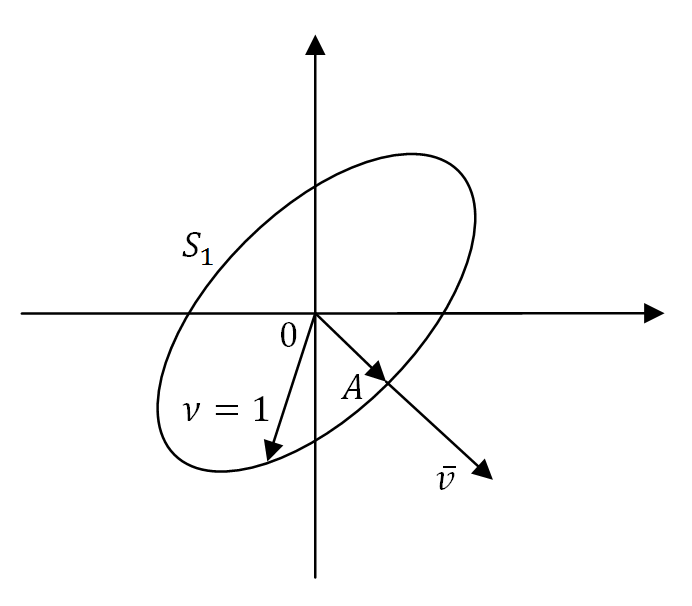
\includegraphics[scale=0.6]{l5_2.png}\\
	$A = $ луч $ \cap S_1$, $~S_1$ --- граница\\
	$\nu(OA) = 1$\\
	$\nu(v) = \lambda \nu(OA) = \lambda$, если $v = \lambda OA, \lambda = \cfrac{|v|}{|OA|}$
\end{center}
\textbf{Лемма.}
Пусть $\nu_1, \nu_2$ --- две нормы на $\mathbb{R}^n$, тогда существует такое $c>0$, что любой шар одной нормы содержится в другом шаре другой нормы.\begin{center}
	$B_R^{\nu_1} \subset B_{cR}^{\nu_2}$.\end{center}
\textbf{Следствие.}
Любые две нормы в $\mathbb{R}^n$ эквивалентны, то есть для $\forall~ \nu_1, \nu_2 ~\exists~ c_1, c_2$, что для $\forall ~\bar x$ верно $c_1\nu_1(x) \leqslant \nu_2(x) \leqslant c_2\nu_1(x)$.\\
\\
\textbf{Следствие.}
Шар $B_1^{\nu_1}$ --- ограниченное множество, то есть $B_R^{\nu_1} \subset \{ \bar x ~|~ |\bar x| \leqslant M \} = B_M^E$ (евклидов шар).\begin{center}
	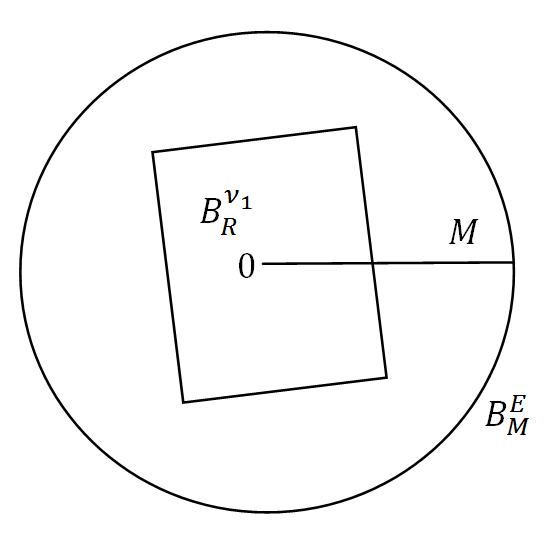
\includegraphics[scale=0.5]{l5_4.png}\end{center}
$\blacktriangleright \nu_2 = $евклидова длина, $M=cR ~~ \blacksquare$\\
\\
\textbf{Доказательство леммы.}\\
$\blacktriangleright$ 
Пусть \[\bar x = \begin{pmatrix}
x_1 \\
...\\
x_n \\
\end{pmatrix} = x_1 \bar e_1 +...+x_n \bar e_n \in B_1^{\nu_1} (R = 1)\]
$\nu_2(\bar x) = \nu_2 (x_1 \bar e_1 +...+x_n \bar e_n) \leqslant \nu_2(x_1e_1)+...+\nu_2(x_ne_n) = |x_1|\nu_2(e_1)+...+|x_n|\nu_2(e_n) \leqslant \\ \leqslant \underset{i=1,...,n}{max} \{\ |x_i|\}$.\begin{center}
	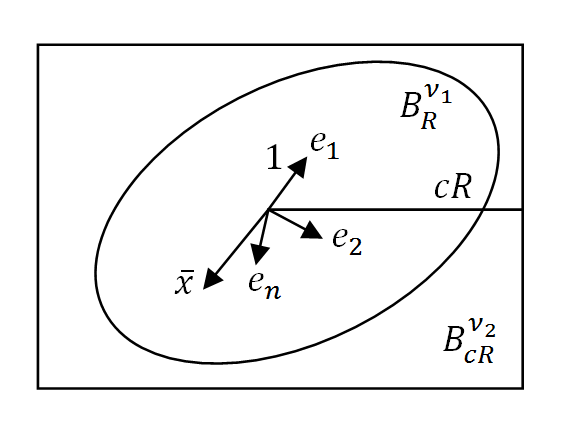
\includegraphics[scale=0.5]{l5_5.png}\end{center}
Пусть $|\bar x|_{\infty} = \underset{i=1,...,n}{max}|x_i|, ~M = \underset{i=1,...,n}{max}\nu_2(e_i)$, тогда $\nu_2(x) \leqslant |\bar x|_{\infty}nM$, то есть $B_R^{\nu_1} \subset B_{cR}^{|\cdot |_{\infty}}, c = nM$.\\
Доказали, что любой единичный шар можно поместить в квадрат со стороной $cR$.\\
\\
Если $|x|_{\infty} \leqslant \cfrac{1}{nM}$, то $\nu_2(x) \leqslant 1, x \in B_1^{\nu_2}$.\begin{center} 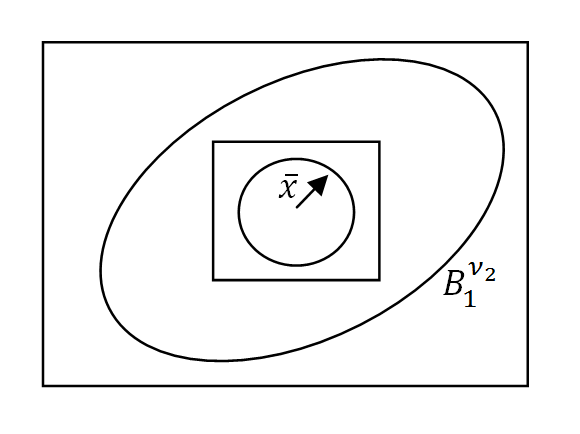
\includegraphics[scale=0.5]{l5_6.png}\end{center}
Внутри любого единичного шара существует квадрат, то есть существует куб, который содержит его целиком. Осталось доказать, что шар --- ограниченное множество. Докажем от противного.\begin{center}
	$B_1^{\nu} = \{x | \nu(\bar x) \leqslant 1\}$\end{center}
Пусть существует $\{x^1, x^2,...\}: \{|x^1|, |x^2|,...\} \rightarrow +\infty$, тогда она существует, если $B_1^{\nu}$ неотрицательное множество.\begin{center}
	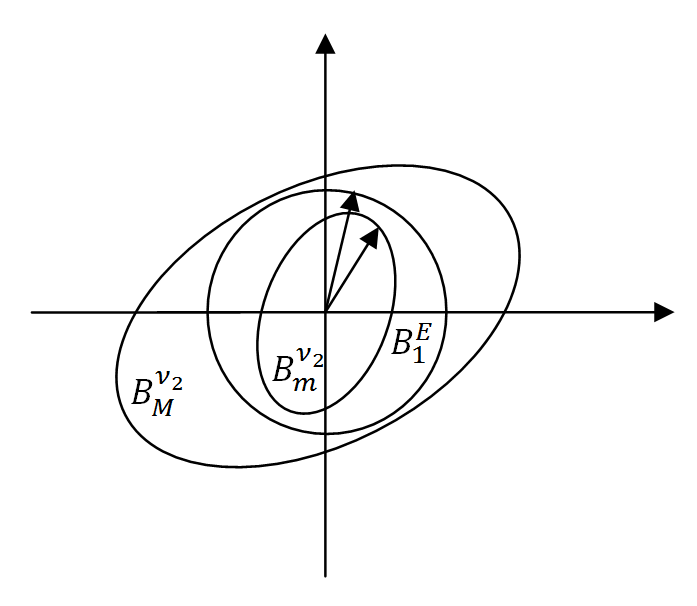
\includegraphics[scale=0.55]{l5_7.png}
	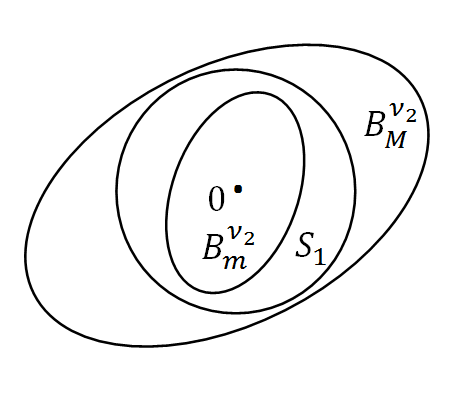
\includegraphics[scale=0.55]{l5_9.png}
	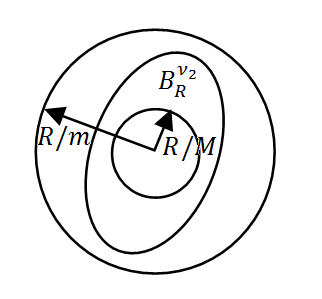
\includegraphics[scale=0.65]{l5_8.png}\end{center}
$m \leqslant \nu_2(B_1^E) \leqslant M$, где $m > 0, ~M$ --- ограниченное множество, тогда (так как все шары подобны):\\ \\
$
\left\{  
\begin{array}{lcl}  
B_m^{\nu_2} \subset B_1^E \subset B_M^{\nu_2} \\  
B_R^{\nu_2} \subset B_{R/m}^E \\
B_{R/M}^E \subset B_R^{\nu_2}\\
\end{array}   
\right.  
$
\\
$\blacksquare$
\\ 
\textbf{Теорема Минковского.}
Множество $B \subset \mathbb{R}^n$ является единичным шаром $B_1^{\nu}$ относительно какой-либо нормы $\nu$ тогда и только тогда, когда $B$:\begin{enumerate}
	\item замкнуто
	\item ограничено ($B \subset B_M^E$)
	\item содержит окрестность нуля (то есть $B \supset B_m^E$)
	\item выпукло
	\item центрально симметрично (если $\bar x \in B$, то и $-\bar x \in B$)
\end{enumerate}
\textbf{Пример 1.}\\
$B = \{x^2+axy+4y^2 \leqslant 1\}$\\
Существует ли такая норма $\nu$, что $B$ --- единичный шар относительно нее ($B = B_1^{\nu}$)?\\
\begin{center}
	$
	\begin{pmatrix}
	1 & \cfrac{a}{2}\\
	\cfrac{a}{2} & 4
	\end{pmatrix}
	$
	\\ ~\\
	$\vartriangle_1 = 1 > 0$\\
	$\vartriangle_2 = 4 - \cfrac{a^2}{4} > 0$\end{center}
То есть это эллипс, все 5 свойств из предыдущей теоремы выполняются, значит при $|a| < 4 B$ --- единичный шар относительно нормы.\begin{center}
	$\vartriangle_1 = 1 > 0$\\
	$\vartriangle_2 = 4 - \cfrac{a^2}{4} < 0$\end{center}
В этом случае множество не будет замкнутым, то есть не выполняются все свойства из предыдущей теоремы, значит в этом случае $B$ не будет единичным шаром относительно нормы.\\
При $\vartriangle_2 = 0$: $ a = \pm 4$ и $x^2 \pm 4xy+4y^2 \leqslant 1$, $(x \pm 2y)^2 \leqslant 1$. В этом случа получим множество между двумя параллельными прямыми, которое является незамкнутым, то есть в этом случае $B$ тоже не будет единичным шаром относительно нормы.\\
Получили, что $B = B_1^{\nu}$ только при $|a| < 4$.\\
\\
$V$ --- \textbf{евклидово пространство со скалярным произведением}, если задана $V \times V \rightarrow \mathbb{R}$, то есть, на нем задано скалярное произведение $(\bar u, \bar v) \in \mathbb{R}$ такое, что для пространств над $\mathbb{R}$ выполнено:\begin{enumerate}
	\item $(u, v) = (v, u)$
	\item $(u'+u'', v) = (u', v)+(u'', v)$
	\item $\alpha (u, v) = (\alpha u, v) = (u, \alpha v), \alpha \in \mathbb{R}$
	\item $(u, u) > 0, u \neq \bar 0~ ((u, u) = 0 \Leftrightarrow u=0)$
\end{enumerate}
Обозначение скалярного произведения: $(u, v)=<u, v>=<u~|~v>$.\\ \\
Длина вектора --- это $|v| = \sqrt{(v, v)} \geqslant 0$ (норма).\\
$\blacktriangleright$ \begin{center}$|\alpha v| = \sqrt{(\alpha v, \alpha v)} = \sqrt{\alpha^2 (v, v)} = |\alpha||v|$\\
	$|v| > 0$, при $v \neq \bar 0$\\
	$|u+v| \leqslant |u|+|v| ~~\blacksquare$\end{center}
$$cos \widehat{(u, v)} = \cfrac{(u, v)}{|u||v|}, u, v \neq \bar 0$$\\
$V$ --- \textbf{эрмитово пространство со скалярным произведением}, если задана $V \times V$ $\rightarrow \mathbb{C}$, то есть, на нем задано скалярное произведение $(\bar u, \bar v) \in \mathbb{C}$ такое, что для пространств над $\mathbb{C}$ выполнено:\begin{enumerate}
	\item $(u, v) = \overline{(v, u)}$
	\item $(u'+u'', v) = (u', v)+(u'', v)$
	\item $\alpha (u, v) = (\alpha u, v) = (u, \alpha v), \alpha \in \mathbb{C}$
	\item $\forall u~ (u, u) \geqslant 0, (u, u) = 0 \Leftrightarrow u=0$
\end{enumerate}
Как по норме $|w|$ восстановить скалярное произведение $(u, v)$?
\begin{center}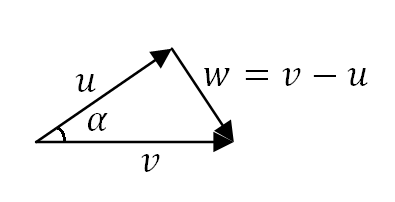
\includegraphics[scale=0.55]{l5_10.png}\\
	$|w|^2 = (w, w) = (v-u, v-u) = (v, v) - (u, v) - (v, u) + (u, u) = |v|^2 - 2(u, v) + |u|^2$\end{center}
То есть, $(u, v) = \cfrac{1}{2}(|v|^2 + |u|^2 - |v-u|^2)$.\\
\\
\textbf{Теорема (тождество параллелограмма).}
Пусть $V$ --- нормированное пространство с нормой $|v|$. На $V$ существует такое скалярное произведение, что $|v| = \sqrt{(v, v)}$ в том и только том случае, когда в $V$ выполняется тождество параллелограмма:\begin{center}
	$\forall a, b~ |a+b|^2 + |b-a|^2 = 2(|a|^2 + |b|^2)$\end{center}
При $c = a+b, d = b-a:$ \begin{center}$c^2+d^2 = 2(a^2+b^2)$\\
	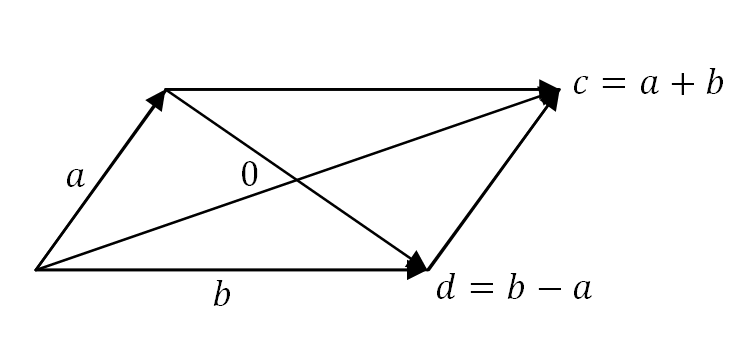
\includegraphics[scale=0.55]{l5_11.png}\end{center}
$\blacktriangleright $ Если для $\forall v ~|v| = \sqrt{<v, v>}$, то $|a+b|^2+|b-a|^2 = <a+b, a+b> + <b-a, b-a> = \\=<a, a> + 2<a, b> + <b, b> +<b, b> - 2<a, b> + <a, a> = 2(|a|^2 + |b|^2)~~ \blacksquare$\\
\\
$H$ --- \textbf{гильбертово пространство}, если на нем задано скалярное произведение и оно является полным (относительно метрики, порожденной скалярным произведением).\\
\\
Набор $\{ \varphi_0, \varphi_1,...,\varphi_n,...\}^{-e}$ называется \textbf{ортогональной системой}, если \\$(\varphi_i, \varphi_j) = \delta_j^i = 
\left\{  
\begin{array}{lcl}  
1, i = j \\  
0, i \neq j \\
\end{array}   
\right.  
$\\
Формально хотим представить $f = \sum\limits_{n=0}^{\infty} c_n \varphi_n$.\begin{center}
	$(f, \varphi_j) = c_j(\varphi_j, \varphi_j)$\\ 
	$(\varphi_j, \varphi_j) = 1$\\ 
	$c_j = \cfrac{(f, \varphi_j)}{\parallel \varphi_j \parallel^2} = (f, \varphi_j)$\end{center} $c_j$ --- коэффициенты Фурье по ортогональной системе.\\ \\
\textbf{Теорема.}
Если $\varphi_j$ --- ортогональная система, тогда следующие условия эквивалентны:\begin{enumerate}
	\item система $\{\varphi_j\}$ является базисом, то есть $f = \sum\limits_{n=0}^{\infty}c_n \varphi_n$
	\item выполнение равенства Парсеваля $\parallel f \parallel^2 = \sum\limits_{n=0}^{\infty}c_k^2$
	\item система является полной, то есть $\exists y \neq 0: (\varphi_j, y) = 0$
\end{enumerate}
Хотим приблизить $f$ и минимизировать $\parallel f - \sum\limits_{k=0}^n \alpha_k \varphi_k \parallel \to min$.\\
$(f - \sum\limits_{k=0}^n \alpha_k \varphi_k, f - \sum\limits_{k=0}^n \alpha_k \varphi_k) =$ (так как система ортогональна) $= (f, f) - 2\sum\limits_{k=0}^n \alpha_k (f, \varphi_k) +\\+\sum\limits_{k=0}^n \alpha_k^2 (\varphi_k, \varphi_k) = (c_k=(f, \varphi_k),~ (\varphi_k, \varphi_k)=1) = \parallel f \parallel^2 + \sum\limits_{k=0}^n (\alpha_k - c_k)^2 - \sum\limits_{k=0}^n c_k^2$\\
Выбором $\alpha$ хотим минимизировать, минимальная норма будет там, где совпадают $\alpha_k = c_k$.\\
\\
$a = \{1, x, x^2,..., x^n\}$ --- пространство $\mathbb{R}_{n+1}$ многочленов степени $\leqslant n$ на $[-1, 1]$, где скалярное произведение $\int\limits_{-1}^1 f(x)g(x)\,dx$. Применим к $a$ процесс Грама-Шмидта, получим $b$.\begin{center}
	$a \to b = \{P_0(x)=1\}$\end{center}
\textbf{Многочлены Лежандра:} \begin{center}$P_k(x) = \cfrac{1}{2^k k!}\cfrac{d^k}{dx^k}((x^2-1)^k)^{(k)}, k=1,..,n$\end{center}\begin{description} 
	\item[k=0:] $P_0(x)=1$
	\item[k=1:] $P_1(x)=\cfrac{1}{2}(x^2-1)'=x$
	\item[k=2:] $P_2(x)=\cfrac{1}{8}((x^2-1)^2)''=\cfrac{1}{8}(4x(x^2-1)'=\cfrac{3x^2-1}{2}$
	\item[k=3:] $P_3(x)=\cfrac{1}{48}((x^2-1)^3)'''=\cfrac{1}{2}(5x^3-3x)$\end{description}
$\parallel P_1(x) \parallel = \sqrt{\int\limits_{-1}^1 x \cdot x\,dx} = \sqrt{\cfrac{2}{3}}$\\
\\
\textbf{Домашнее задание 5}\begin{enumerate}
	\item
	\begin{enumerate}
		\item Проверить ортогональность $P_2(x)$ и $P_3(x)$ относительно $<f, g> =\\= \int\limits_{-1}^1 f(x)g(x)\,dx$.
		\item Найти $\parallel P_n(x) \parallel$.
	\end{enumerate}
	\item
	Найти $\alpha_0, \alpha_1, \alpha_2$ на $[-1, 1]$: $\parallel f - \sum\limits_{k=0}^2 \alpha_kP_k(x) \parallel \to min$, $d_j=\cfrac{(f, \varphi_j)}{\parallel \varphi_j \parallel^2} = (f, \varphi_j)$, где $P_k(x)=\cfrac{1}{2^k k!}\cfrac{d^k}{dx^k}((x^2-1)^k)^{(k)},~k=1,\cdots, n$ --- многочлены Лежандра.
	\begin{enumerate}
		\item $f_1(x)=xe^{-x}$
		\item $f_2(x)=x^3$\\
	\end{enumerate}
	\item
	Выразить скалярное произведение через длину вектора в эрмитовом пространстве.\end{enumerate}


\subsection{Норма}

\subsection{Теорема Минковского}


\newpage
\section{Многочлены Чебышева}

\newpage
\section{Матричные нормы}












\end{document}